\documentclass{article}

%%%%%%%%%%%%%%%%%%%%%%%%%%%%%%%%
% PACKAGES
%%%%%%%%%%%%%%%%%%%%%%%%%%%%%%%%
\usepackage{times}
\usepackage{fullpage}
\usepackage{latexsym}
\usepackage{amsmath}
\usepackage{amssymb}
\usepackage{mathtools}
\usepackage{accents}
\usepackage{tikz}
\usepackage{pgfplots}
\usepackage[ruled]{algorithm}
\usepackage{algpseudocode}
\usepackage{dsfont}
\usepackage[bf]{caption}
\usepackage{hyperref}
\hypersetup{
    bookmarks=true,         % show bookmarks bar?
    unicode=false,          % non-Latin characters in AcrobatÕs bookmarks
    pdftoolbar=true,        % show AcrobatÕs toolbar?
    pdfmenubar=true,        % show AcrobatÕs menu?
    pdffitwindow=false,     % window fit to page when opened
    pdfstartview={FitH},    % fits the width of the page to the window
    pdftitle={My title},    % title
    pdfauthor={Author},     % author
    pdfsubject={Subject},   % subject of the document
    pdfcreator={Creator},   % creator of the document
    pdfproducer={Producer}, % producer of the document
    pdfkeywords={keyword1} {key2} {key3}, % list of keywords
    pdfnewwindow=true,      % links in new window
    colorlinks=true,       % false: boxed links; true: colored links
    linkcolor=red,          % color of internal links (change box color with linkbordercolor)
    citecolor=blue,        % color of links to bibliography
    filecolor=magenta,      % color of file links
    urlcolor=cyan           % color of external links
}
\usepackage{amsthm}
\usepackage{natbib}
\usepackage[capitalize]{cleveref}
\usepackage{graphicx}
\usepackage{parskip}


\usetikzlibrary{arrows,positioning,backgrounds} 
\tikzset{
    %Define standard arrow tip
    >=stealth',
    %Define style for boxes
    observed/.style={
           circle,
           rounded corners,
           draw=black, thick,
           minimum width=2.2em,
           minimum height=2.2em,
           font=\tiny,
           text centered,
           scale=.8,
           fill=blue!20!white},
     latent/.style={
           circle,
           rounded corners,
           draw=black, thick, dashed,
           minimum width=.5em,
           minimum height=.5em,
           font=\footnotesize,
           text centered,
           fill=black!10!white
           },
     empty/.style={
           circle,
           rounded corners,
           minimum width=.5em,
           minimum height=.5em,
           font=\footnotesize,
           text centered,
           },
    % Define arrow style
    pil/.style={
           o->,
           thick,
           shorten <=2pt,
           shorten >=2pt,},
    sh/.style={ shade, shading=axis, left color=red, right color=green,
    shading angle=45 }  
}

%%%%%%%%%%%%%%%%%%%%%%%%%%%%%%%%
% MACROS
%%%%%%%%%%%%%%%%%%%%%%%%%%%%%%%%
\newcommand{\defined}{\vcentcolon =}
\newcommand{\rdefined}{=\vcentcolon}
\newcommand{\E}{\mathbb E}
\newcommand{\Var}{\operatorname{Var}}
\newcommand{\calF}{\mathcal F}
\newcommand{\sr}[1]{\stackrel{#1}}
\newcommand{\set}[1]{\left\{#1\right\}}
\newcommand{\ind}[1]{\mathds{1}\!\!\set{#1}}
\newcommand{\argmax}{\operatornamewithlimits{arg\,max}}
\newcommand{\argmin}{\operatornamewithlimits{arg\,min}}
\newcommand{\floor}[1]{\left \lfloor {#1} \right\rfloor}
\newcommand{\ceil}[1]{\left \lceil {#1} \right\rceil}
\newcommand{\eqn}[1]{\begin{align}#1\end{align}}
\newcommand{\eq}[1]{\begin{align*}#1\end{align*}}
\newcommand{\Ber}{\operatorname{Bernoulli}}
\renewcommand{\P}[1]{\operatorname{P}\left\{#1\right\}}
\newcommand{\pt}{\mathcal P}


%%%%%%%%%%%%%%%%%%%%%%%%%%%%%%%%
% THEOREMS
%%%%%%%%%%%%%%%%%%%%%%%%%%%%%%%%
\theoremstyle{plain}
\newtheorem{theorem}{Theorem}
\newtheorem{proposition}[theorem]{Proposition}
\newtheorem{lemma}[theorem]{Lemma}
\newtheorem{corollary}[theorem]{Corollary}
\theoremstyle{definition}
\newtheorem{definition}[theorem]{Definition}
\newtheorem{assumption}[theorem]{Assumption}
\newtheorem{remark}[theorem]{Remark}
\newtheorem{example}[theorem]{Example}

\title{Protecting causal effects}
\author{}

\begin{document}
\def\ci{\perp\!\!\!\perp}
\maketitle

Differential privacy has primarily focused on protecting individuals but there is increasing interest in problems relating to hiding certain aggregate properties of a dataset whilst preserving the ability to use it for a specified purpose. In this problem we consider if we can release a dataset for predictive purposes but discourage the inference of causal conclusions about relationships between the covariates. 

Consider a scenario under which the causal graph generating a dataset is considered known - but may contain unmeasured variables. 

Assume we add noise to the dataset via a single point crossover process (see paper). The goal is to prevent reliable estimation of causal effects without effecting our ability to predict a particular target variable. Some example questions:

\begin{itemize}
\item Under what circumstances (graph structures) it is possible to disrupt inference of a particular causal effect \textcolor{red}{always provided there is a direct causal relationship between the exposure variable $X$ and outcome variable $Y$, ie $P(Y|do(X))\neq P(Y)$} 
\item How can we maxiumully disrupt this inference (ie is there a cut that adds more noise for a given amount of shuffling of the data) \textcolor{red}{data dependent}
\item What about if we want to disrupt a specific set of causal inference questions
\item What about if we want to disrupt as many causal queries as possible.
\end{itemize}

\section{Problem Statement and Definitions}

\begin{itemize}
\item Let $G$ be a causal directed acyclic graph over vertices $V$ and edges $E$.
\item Let $S = \set{(X_1,Y_1),(X_2,Y_2),...,(X_m,Y_m): X_i,Y_i \in V,X_i \neq Y_i}$ be a set of pairs of vertices in $G$.
\item Each pair of vertices $(X_i,Y_i)$ in $S$ represents the causal query $P(Y_i|do(X_i))$
\item A set of variables $Z \subset V$ is an adjustment for a query $(X,Y)$ if $X, Y \notin Z$ and $P(Y|do(X)) = \sum_Z P(Y|X,Z)P(Z)$
\item An adjustment for a query is minimal if it does not contain another adjustment as a proper subset.
\item The Single Point Crossover Process partitions the variables $V$ into two disjoint sets, $\pt_1$ and $\pt_2$ such that $\pt_1 \cup \pt_2 = V$. Let $\pt_X$ denote the partition containing the variable $X$.
\end{itemize}

\subsection{Discouraging inference of a set of causal queries via adjustment}

%Causal effects differ from non-causal ones due to bias introduced by confounding variables, which effect both treatment assignment and outcome. For example, ...

Adjusting for nuisance or confounding variables, either by matching or regression, has been a key technique in inferring causal effects at least as far back as \cite{}. The widely used back-door criterion \cite{Pearl2000} clarifies which variables it is appropriate to condition on in order to achieve unbiased estimates of causal effects. 

\begin{lemma}Where $X$ and $Y$ are singleton variables, $Z$ is a minimal covariate adjustment for identifying the causal effect of $X$ on $Y$ if and only if $Z$ is a minimal set satisfying the backdoor-criterion relative to $X$ and $Y$ \cite{textor2012adjustment}.
\end{lemma}
 
The existence of a set covariate adjustment is sufficient but not necessary for identifiability. A causal query can also be identified 


We will consider non-parametric point identifiability as described by \cite{Pearl2000}. 

The do-calculus provides a complete framework to determine if and how a causal effect may be  identified from observational data. The framework assumes that the data is generated by a directed acyclic graph (DAG) and that the structure of the graph is known (although some variables may not be observed). 

is a sufficient criterion for identification of causal effects via matching. More recently it has been generalized to provide necessary and sufficient critera for identification via matching for DAGs \cite{}, and MAGs PAGs \cite{}. 

More recently, \cite{Pearl2000} developed the do-calculus, which provides a complete framework for determining if a causal query can be identified from observational data. 




\begin{definition}
Identifiability. 
A query $P(Y|do(X))$ is identifiable in a causal graph $G$ if it can be computed uniquely from any positive probability distribution over the observed variables - that is, we can compute an expression for $P(Y|do(X))$ that contains only factors of the observed distribution. 
\end{definition}
\begin{enumerate}
\item $P(Y|do(X)) = P(Y)$. 
\label{cat:noncausal}
\item $P(Y|do(X)) = \sum_Z P(Y|X,Z)P(Z)$
\label{cat:adjust}
\item $P(Y|do(X))$ is identifiable but not via (1) or (2)
\label{cat:identify_other}
\item $P(Y|do(X))$ is not identifiable
\label{cat:not_identifiable}
\end{enumerate}


In this paper we focus on jamming queries that fall into case \ref{cat:adjust}. Case \ref{cat:noncausal} cannot be jammed as the SPCP does not modify marginal distributions. However, it is also unlikely to be sensitive as it holds only if there is no casual relationship between $X$ and $Y$. In case \ref{cat:not_identifiable}, the causal effect cannot be identified from this data set so there is no further work required to jam it. Case \ref{cat:identify_other} is complex and rarely used in empirical work. We leave it for future work.

\begin{lemma}Let $Z$ be a set of variables that is a minimal adjustment for the causal query $(X,Y)$. Inferring $P(Y|do(X))$ via adjusting for $Z$ is jammed if $Y \cup Z \not\subset \pt_X$. In other words, if at least one of the variables in $X \cup Y \cup Z$ is in a different a different partition to the others. 

Note: this holds only if $Z$ is a \textit{minimal} adjustment. If $Z$ is not minimal then we can let $Z = Z' \cup U$ where $Z'$ is a minimal adjustment. In this case, we can still estimate the causal effect of $X$ on $Y$ by conditioning on $Z'$. 

\color{red} This stems from the fact that the expression for calculating $P(Y|do(X))$ via adjusting for $Z$ contains the factor $P(Y|X,Z)$.  I'm assuming the single point crossover process gives us this result. We need to a clear definition of 'jammed' in terms of the crossover-process.
\end{lemma}

\begin{lemma} Let $\boldsymbol{Z}$ be the set of minimal adjustments for $(X,Y)$. The causal query $(X,Y)$ is jammed if inferring $P(Y|do(X))$ via $Z$ is jammed for $\forall Z \in \boldsymbol{Z}$ 
\end{lemma}


\subsubsection{An algorithm for finding a cut that renders jams a set of causal queries $S$}
\begin{enumerate}
\item For each query $(X_i,Y_i)\in S$, find the set of minimal adjustments $\boldsymbol{Z}_i$  
\item Construct the set of sets $Q = \set{X_i \cup Y_i \cup Z_{ik} : 1 \leq i \leq m, 0 \leq k \leq |\boldsymbol{Z}_i|}$
\item Find a partition such that $(Q_i \nsubseteq \pt_1)\land (Q_i \nsubseteq \pt_2)\qquad \forall Q_i \in Q$
\end{enumerate}

For example in figure \ref{fig:minimal_sets_example}, with $S = \set{(A,B),(E,B),(C,B),(E,A)}$

\eq{
&S_1 = (A,B),\, \boldsymbol{Z}_1 = \set{\set{C, E},\set{D,E} \set{D,F}} \\
&S_2 = (E,B),\, \boldsymbol{Z}_2 = \set{\set{C,D}} \\
&S_3 = (C,B),\, \boldsymbol{Z}_3 = \set{} \\
&S_4 = (E,A),\, \boldsymbol{Z}_4 = \set{C} \\
&Q = \set{\set{A,B,C,E},\set{A,B,D,E},\set{A,B,D,F},\set{E,B,C,D},\set{C,B},\set{E,A,C}}
}


We could jam $S$ with any partition of the form $\set{A,B,...},\set{C,E,F,...}$.$S_2,S_3$ and $S_4$ are jammed because their $X$ and $Y$ variables are in different partitions. $S_1$ is jammed because, although $A$ and $B$ are in the same partition, for each of the three minimal adjustment sets, at least one variable is not in $\pt_A$. $D$ could be placed in either partition. This is not the only solution, $\set{A,C,...},\set{B,E,...}$ is another. Note than in any solution $B$ and $C$ must be in different partitions as this is the only way to jam $S_3$.

The number of minimal adjustments for a given query can grow exponentially with the number of nodes in the graph. There is an algorithm to enumerate them that requires $O(n^3)$ per adjustment \cite{textor2012adjustment} .


\begin{figure}
\caption{}
\label{fig:minimal_sets_example}
\centering
   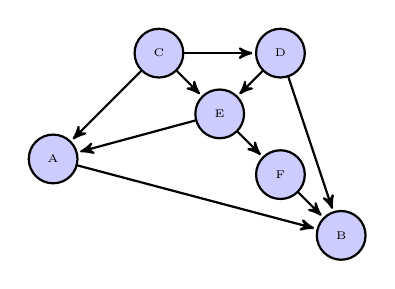
\begin{tikzpicture}[->,>=stealth',shorten >=1pt,auto,node distance=.45cm,
  thick,main node/.style={observed}, hidden/.style={empty},background rectangle/.style={fill=olive!45}]
%every node/.style={scale=0.6}
 %nodes
\node[main node](1){C};
\node[main node, below right=of 1](3){E};
\node[main node, above right=of 3](2){D};
\node[main node, below right=of 3](4){F};
\node[main node, below right=of 4](5){B};
\node[hidden, below left=of 1](7){};
\node[main node, below left=of 7](6){A};
 \path[every node/.style={font=\tiny}]
    (1) edge (2) edge (3) edge (6)
    (6) edge (5)
    (2) edge (3) edge (5)
    (3) edge (4) edge (6)
    (4) edge (5);
\end{tikzpicture}
\end{figure}



\subsubsection{Some things we can say}

\begin{itemize}
\item If $\boldsymbol{X} = \set{X_1 ... X_m}$ and $\boldsymbol{Y} = \set{Y_1...Y_m}$ are disjoint sets, then any partition with $\boldsymbol{X} \subseteq \pt_1$ and $\boldsymbol{Y} \subseteq \pt_2$ will jam $S$. This holds trivially if $|S|$ = 1.
\item The hardest case to jam is when $\boldsymbol{Z}_i = {} \forall i$
\item If $|S| = 2$ we can always jam $S$ as either $\boldsymbol{X}$ and $\boldsymbol{Y}$ will be disjoint or a variable $A$ will appear in both $S_1$ and $S_2$, in which case we can let $\pt_1 = \set{A}$.
\end{itemize}

\subsection{Further work}

We have considered only single variable interventions and outcomes. We believe the results generalize in a straightforwardly to the case where, for each causal query, $X$ and $Y$ are sets with a minor assumption that there are no causal paths from one intervention variable $X$ to another.

Although overwhelmingly used in practice, adjustment is not necessary for causal identifiability. A given causal graph may also be identifiable via the front door criterion \cite{} or via an expression returned by the identify algorithm \cite{}. 

What is the psuedo code to jam all mechanisms? We need an algorithm to produce all 'minimal' expressions. Then each expression will contain a set of factors. At least one of those factors must be jammed for every expression. 

Note: A given query may be identifiable via multiple different expressions. As we must jam all of them, it is not sufficient to have an algorithm that returns \textit{an} expression (if one exists). We are not aware of any such algorithms for the general identifiability problem. 

Prove that a single query can still always be jammed by separating $X$ and $Y$. Approach  - the expression is a result of the do calculus and nessesarily contains a term with both $X$ and $Y$ together unless... 

\bibliographystyle{apalike}
\bibliography{/home/finn/phd/Causality-Identify}

\end{document}




